\chapter{Consideraciones importantes}
\label{apendiceA}
\lhead{Apéndice A.}

En el presente apéndice se exponen elementos importantes de considerar al momento de trabajar con el OpenROV. 

\section{Baterías}
\par El OpenROV está diseñado para usar baterias de Litio 26650(26.5mm × 65.4mm). Inicialmente usaba unas Li-FePO4, 3300mAh y 3.2V. Durante el desarrollo de este proyecto una batería (R2) resultó dañada y otra (L1) empezó a tener un desempeño, algunas veces, deficiente. Sin embargo, todavía es posible manipular el robot utilizando únicamente uno de los dos tubos con tres baterías. 

\par Por otra parte, nuevas baterías fueron adquiridas, pero estas difieren en la química de las baterías previas. Son unas recargables Li-MN 4200MAH, \textit{High Drain} 60A de 3.7V.

\subsection{Configuración de las baterías}
\par Al abrir el cockpit es importante indicar con cuales baterías se está trabajando y establecer una configuración para ellas, de manera que se pueda saber el nivel de voltaje y cuanta energía le queda al robot.

En la sección \textit{Settings} -$>$ \textit{Battery Configuration}, se selecciona o agregan las baterías que están en uso. Por defecto, al descargar la imagen del OpenROV ya vienen incluidas las Li-FeP04. Para las nuevas baterías es importante introducir el nombre de la química de la batería, la  tensión máxima y la tensión mínima.

    \begin{figure}[H]
        \centering
        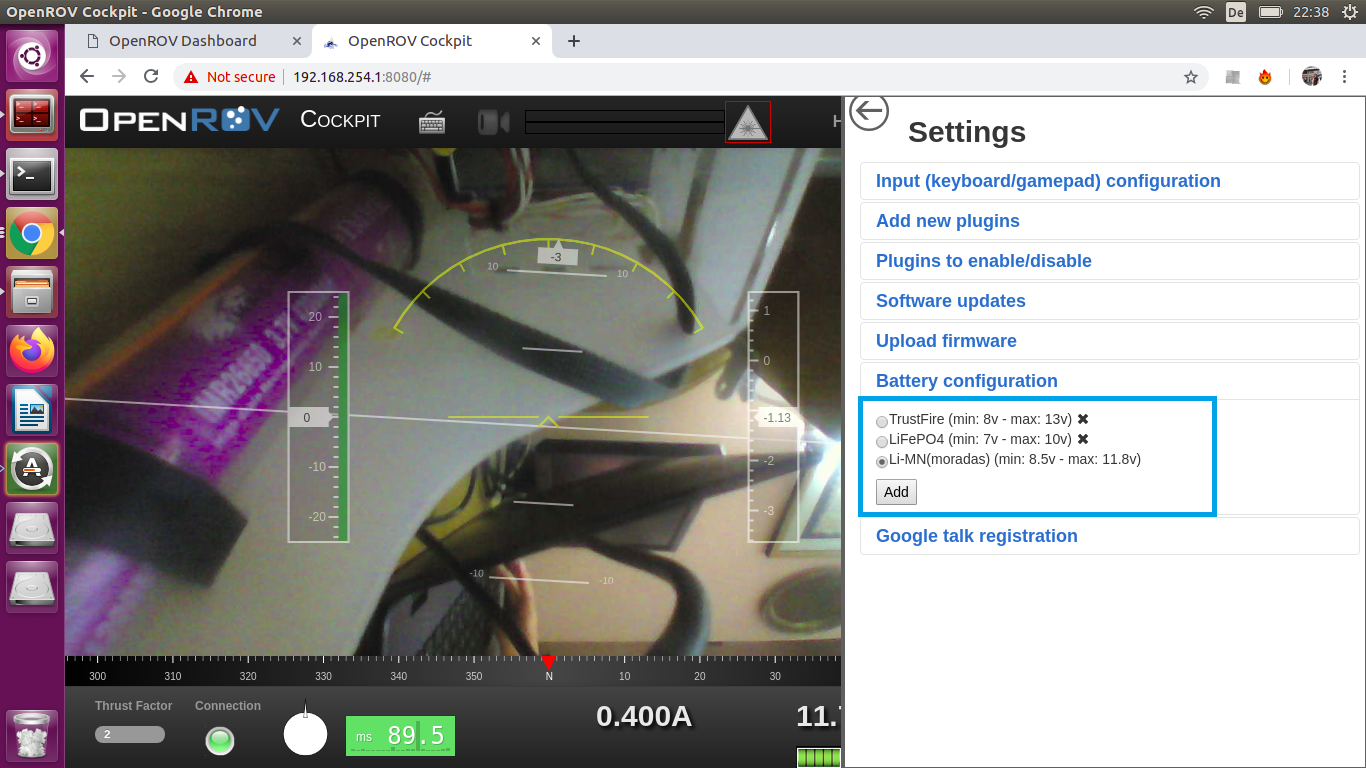
\includegraphics[scale=0.4]{partes/ImgSophia/Apendice/Baterias.png}
        \caption{Configuración de las baterías en el cockpit}
        \label{fig:BattCockpit}
    \end{figure}

\subsection{Carga de las baterías}
La configuración del cargador difiere dependiendo de la batería con la que se esté trabajando y debe ser ajustado de la siguiente forma:

\begin{table}[H]
\caption {Características de las baterías} 
\label{tab:batt}
\centering
\begin{tabular}{@{}ccccc@{}}
\toprule
\textbf{Batería}  & \begin{tabular}[c]{@{}c@{}}\textbf{Conf. Cargador} \\ {[}V{]}\end{tabular} & \begin{tabular}[c]{@{}c@{}}\textbf{Voltaje nominal}\\ {[}V{]}\end{tabular} & \begin{tabular}[c]{@{}c@{}}\textbf{Capacidad}\\ {[}mAh{]}\end{tabular} & \textbf{Color}  \\ \midrule
Li-FePO4 & 3.0      & 3.2       & 3300      & Blanco \\
Li-MN    & 4.2      & 3.7       & 4200       & Morado \\ \bottomrule
\end{tabular}
\end{table}

\section{Conexión a Internet: interfaces usb0 y eth0}


El cerebro del OpenROV es el BeagleBone Black, que posee dos interfaces que facilitan establecer la comunicación con un equipo externo. Pueden ser revisadas en \verb|$ sudo cat /etc/network/interfaces| y son:

\begin{itemize}
    \item Interfaz usb0, con la IP : 192.168.7.2, para el protocolo $SSH$
    \item Interfaz eth0, con la IP estática : 192.168.254.1 en la que está construida el cockpit.
\end{itemize}

Es importante que después de realizar cualquier modificación en ese archivo, las redes sean reiniciadas con: \verb|$ sudo /etc/init.d/networking restart|

\begin{table} [H]
\caption {Interfaces usb0 y eth0 definidas en el OpenROV} 
\label{tab:usb0eth0}
\centering
\begin{tabular}{@{}lll@{}}
\toprule
\multicolumn{1}{c}{\textbf{Interfaz}} & \multicolumn{1}{c}{\textbf{usb0}} & \multicolumn{1}{c}{\textbf{eth0}} \\ \midrule
IP estática         & 192.168.7.2       & 192.168.254.1           \\
red                 & 192.168.7.0       & 192.168.254.0            \\
\textit{gateway}    & 192.168.7.1       & 192.168.254.254           \\ 
\textit{broadcast}  & \multicolumn{1}{c}{/} & 192.168.254.255        \\ \bottomrule
\end{tabular}
\end{table}

\subsection{\textit{SSH}}
El comando ssh ofrece una comunicación segura con el OpenROV. La primera vez que se intenta iniciar sesión es necesario aceptar la firma de este otro host (OpenROV). Si se está en windows el ssh se puede realizar usando PuTTY; en linux se puede realizar directamente desde el terminal.

La sintaxis básica es: \verb|ssh user@hostname|, en este caso \verb|$ ssh rov@192.168.7.2|.

\begin{table} [H]
\caption {Datos por defecto para iniciar sesión en el OpenROV} 
\label{tab:UserPass}
\centering
\begin{tabular}{@{}ll@{}}
\toprule
Usuario    & OpenROV \\ \midrule
Contraseña & OpenROV \\ \bottomrule
\end{tabular}
\end{table}

\subsection{Conexión a internet}

La conexión a internet del BeagleBone Black se puede hacer usando un cable USB (interfaz usb0) o a través de un cable Ethernet (interfaz eth0). Dependiendo del caso es necesario tomar las siguiente consideraciones: 

\subsubsection{Interfaz usb0.}
    \begin{itemize}
        \item Conectar el BeagleBone a un puerto USB de la computadora
        \item Instalar los drivers necesarios.
        \item En control panel, configuracion del adaptado: fijar la IP del puerto USB a 192.168.7.1 (para que coincida con el gateway del BBB)
        \item En el adaptador que tiene la conexion a internet es necesario habilitar el compartir la conexión con el puerto USB que será el gateway.
        \item Realizar $ssh$ al BeagleBone (\verb|$ ssh rov@192.168.7.2|). 
        \item Es necesario ejecutar el comando: \verb|$ route add default gw 192.168.7.1|
        \item Además se puede agregar el servidor de Google en \verb|$ cd /etc/resolv.conf| colocando la línea "nameserver 8.8.8.8"
        \item Para verificar la conexión con el computador es recomendable enviar desde el BBB un \verb|$ ping 192.168.7.1|
        \item Para verificar la conexión a internet: \verb|$ wget --no-proxy google.com|
    \end{itemize}
    
\subsubsection{Interfaz eth0}
    \begin{itemize}
        \item Conectar un cable directamente del BeagleBone Black al router.
        \item Realizar $ssh$ al BeagleBone (\verb|$ ssh rov@192.168.7.2|).
        \item Abrir las interfaces de red: \verb|$ sudo nano /etc/network/interfaces|
        \item Comentar las líneas donde se establece la dirección estática IP 192.168.254.1 y los otros parámetros de esta interfaz tal como: gateway, red, broadcast. 
        \item Agregar una nueva interfaz: iface eth0 inet dhcp y guardar los cambios. Esto ya debería garantizar tener una conexion a internet operativa, sin embargo, es un problema si se quiere realizar ssh por este medio en próximas ocasiones ya que esa IP es asignada aleatoriamente.
        \item Garantizar que los cambios sean ejecutados:
        
        \verb|$ sudo /etc/init.d/networking restart|
        \item Se procede a fijar la IP obtenida de forma estática. Para visualizar la IP y los nuevos parámetros de esa interfaz se usa:
        
\begin{verbatim}
$ ip addr show | grep eth0
\end{verbatim}
        \item Nuevamente \verb|$ sudo nano /etc/network/interfaces|, se cambia dhcp por static y se agregan: $addres, netmask, gateway$ y, preferiblemente los dos dns de google: $dns-nameservers$ 8.8.8.8 y 8.8.4.4
        \item Agregar \verb|nameserver 8.8.8.8| en \verb|$ sudo nano /etc/resolv.conf| 
        \item Deshabilitar el proxy: \verb|$ sudo /etc/init.d/openrov-proxy stop| 
        \item Para verificar la conexión a internet \verb|$ sudo ping google.com|
        \item Si se presenta algún problema probar \verb|$ wget --no-proxy google.com|
    \end{itemize}

\subsection{Problemas conectando a internet}

\par A pesar de obtener resultados satisfactorios en un primer momento realizando la conexión a internet usando la interfaz usb0, hubo un punto en el que al revisar la tabla de enrutamiento IP, no se encontraban los gateways de las redes predefinidas en el OpenROV para eth0 y usb0 \ref{fig:routeIP}.

\begin{figure}[H]
    \centering
    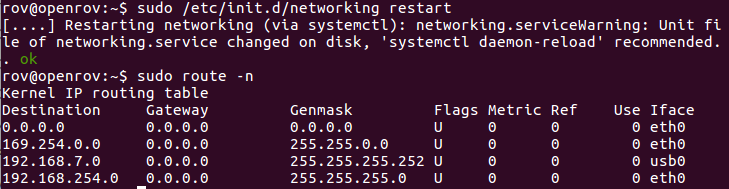
\includegraphics[scale=0.6]{partes/ImgSophia/Apendice/IProutetable.png}
    \caption{Tabla de enrutamiento IP}
    \label{fig:routeIP}
\end{figure}

\par Por esto es \textbf{recomendable} conectar a internet mediante la interfaz eth0 haciendo uso inicialmente del protocolo DHCP, tal como se explicó anteriormente. De esta manera no se presentó ningún incoveniente y con la nueva red agregada se incorporaba el valor fijado para el gateway. 

\subsection{Descarga de dependencias o librerías}

\subsubsection{Error sudo apt-get update}

Al realizar las actualizaciones, se puede obtener el error \verb|503 Service Unavailable| es producto de un problema con el proxy que puede ser resuelto deteniéndolo con: 
\verb|$ sudo /etc/init.d/openrov-proxy stop|

\begin{figure}[H]
    \centering
    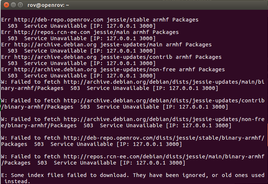
\includegraphics[scale=1.2]{partes/ImgSophia/Apendice/error503.png}
    \caption{Error inicial al sudo apt-get update}
    \label{fig:ErrSudoApt}
\end{figure}

\subsubsection{Errores por falta de actualizaciones de Debian 8 Jessie} 

En la última versión estable del software del OpenROV 2.8: v30.0.3, el sistema operativo de Linux fue actualizado a Linux Debian "Jessie". Sin embargo, actualmente para la version Debian 8 "Jessie", jessie-updates fue removido y jessie-backports archivado en fecha 24-03-2019. La solución es actualizar, de la siguiente manera, el \verb|source.list| a los siguientes suits:

\begin{enumerate}
    \item Abrir el source.list: \verb|$ sudo nano /etc/apt/sources.list| que se corresponde al que se observa en la figura a la continuación:
    
    \begin{figure}[H]
        \centering
        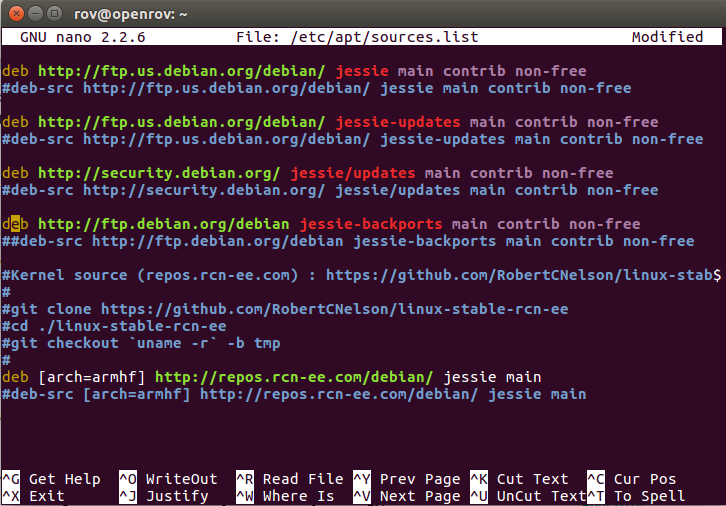
\includegraphics[scale=0.5]{partes/ImgSophia/Apendice/2SourceListOriginal.png}
        \caption{Source.list original del software del OpenROV}
        \label{fig:SourceOriginal}
    \end{figure}
    
    \item Debería ser suficiente con comentar las líneas que contengan jessie-updates (no jessie/updates) y jessie-backports, sin embargo, se recomienda comentar los \textit{suites} presentes y agregar los siguientes: 
    
\footnotesize
\begin{verbatim}
deb http://ftp.debian.org/debian jessie main
deb-src http://ftp.debian.org/debian jessie main

deb http://security.debian.org/debian-security jessie/updates main
deb-src http://security.debian.org/debian-security jessie/updates main

deb http://ftp.debian.org/debian/ jessie-backports main contrib non-free
deb-src http://ftp.debian.org/debian/ jessie-backports main contrib non-free

\end{verbatim}


\normalsize
    \item El \verb|source.list| que funciona queda como se muestra en la figura \ref{fig:SourceFunciona}; hasta este paso fue suficiente para no tener errores con \verb|sudo apt-get update| y poder descargar sin problemas las librerías.
    
    \begin{figure}[H]
        \centering
        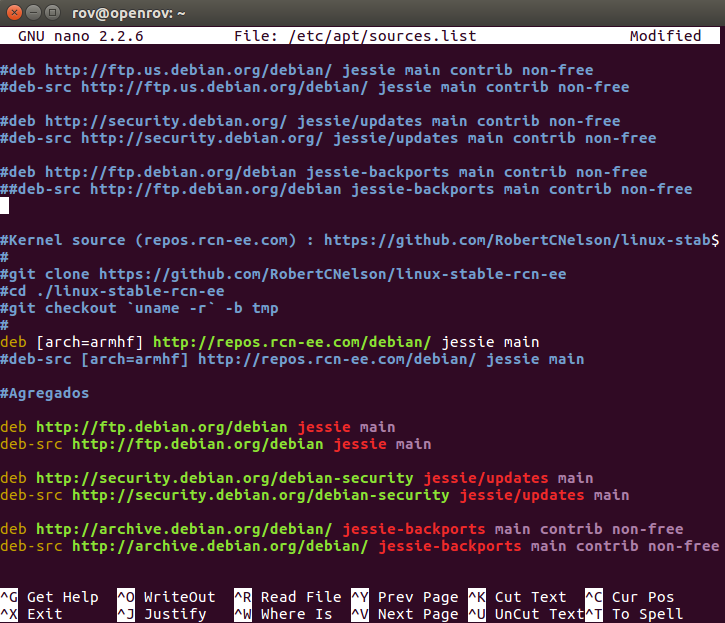
\includegraphics[scale=0.5]{partes/ImgSophia/Apendice/3SourceListFuncional.png}
        \caption{Source.list funcional}
        \label{fig:SourceFunciona}
    \end{figure}
    
    \item Sin embargo, el jessie-backports archivado en  archive.debian.org, debería generar otro error, que de presentarse se solucionaría con:
\end{enumerate}
    \footnotesize
    \verb|echo 'Acquire::Check-Valid-Until no;' > /etc/apt/apt.conf.d/99no-check-valid-until|
\normalsize



